% Options for packages loaded elsewhere
\PassOptionsToPackage{unicode}{hyperref}
\PassOptionsToPackage{hyphens}{url}
%
\documentclass[
]{book}
\usepackage{amsmath,amssymb}
\usepackage{lmodern}
\usepackage{ifxetex,ifluatex}
\ifnum 0\ifxetex 1\fi\ifluatex 1\fi=0 % if pdftex
  \usepackage[T1]{fontenc}
  \usepackage[utf8]{inputenc}
  \usepackage{textcomp} % provide euro and other symbols
\else % if luatex or xetex
  \usepackage{unicode-math}
  \defaultfontfeatures{Scale=MatchLowercase}
  \defaultfontfeatures[\rmfamily]{Ligatures=TeX,Scale=1}
\fi
% Use upquote if available, for straight quotes in verbatim environments
\IfFileExists{upquote.sty}{\usepackage{upquote}}{}
\IfFileExists{microtype.sty}{% use microtype if available
  \usepackage[]{microtype}
  \UseMicrotypeSet[protrusion]{basicmath} % disable protrusion for tt fonts
}{}
\makeatletter
\@ifundefined{KOMAClassName}{% if non-KOMA class
  \IfFileExists{parskip.sty}{%
    \usepackage{parskip}
  }{% else
    \setlength{\parindent}{0pt}
    \setlength{\parskip}{6pt plus 2pt minus 1pt}}
}{% if KOMA class
  \KOMAoptions{parskip=half}}
\makeatother
\usepackage{xcolor}
\IfFileExists{xurl.sty}{\usepackage{xurl}}{} % add URL line breaks if available
\IfFileExists{bookmark.sty}{\usepackage{bookmark}}{\usepackage{hyperref}}
\hypersetup{
  hidelinks,
  pdfcreator={LaTeX via pandoc}}
\urlstyle{same} % disable monospaced font for URLs
\usepackage{longtable,booktabs,array}
\usepackage{calc} % for calculating minipage widths
% Correct order of tables after \paragraph or \subparagraph
\usepackage{etoolbox}
\makeatletter
\patchcmd\longtable{\par}{\if@noskipsec\mbox{}\fi\par}{}{}
\makeatother
% Allow footnotes in longtable head/foot
\IfFileExists{footnotehyper.sty}{\usepackage{footnotehyper}}{\usepackage{footnote}}
\makesavenoteenv{longtable}
\usepackage{graphicx}
\makeatletter
\def\maxwidth{\ifdim\Gin@nat@width>\linewidth\linewidth\else\Gin@nat@width\fi}
\def\maxheight{\ifdim\Gin@nat@height>\textheight\textheight\else\Gin@nat@height\fi}
\makeatother
% Scale images if necessary, so that they will not overflow the page
% margins by default, and it is still possible to overwrite the defaults
% using explicit options in \includegraphics[width, height, ...]{}
\setkeys{Gin}{width=\maxwidth,height=\maxheight,keepaspectratio}
% Set default figure placement to htbp
\makeatletter
\def\fps@figure{htbp}
\makeatother
\setlength{\emergencystretch}{3em} % prevent overfull lines
\providecommand{\tightlist}{%
  \setlength{\itemsep}{0pt}\setlength{\parskip}{0pt}}
\setcounter{secnumdepth}{5}
\usepackage{booktabs}
\ifluatex
  \usepackage{selnolig}  % disable illegal ligatures
\fi
\usepackage[]{natbib}
\bibliographystyle{plainnat}

\author{}
\date{\vspace{-2.5em}2022-03-07}

\begin{document}

{
\setcounter{tocdepth}{1}
\tableofcontents
}
\hypertarget{calvo-cocina}{%
\chapter*{Calvo Cocina}\label{calvo-cocina}}
\addcontentsline{toc}{chapter}{Calvo Cocina}

\emph{Última actualización: 07/03/2022.}


\includegraphics{images/xkcd.png}

\hypertarget{pollo-teriyaki}{%
\chapter{Pollo teriyaki}\label{pollo-teriyaki}}

\begin{figure}
\centering
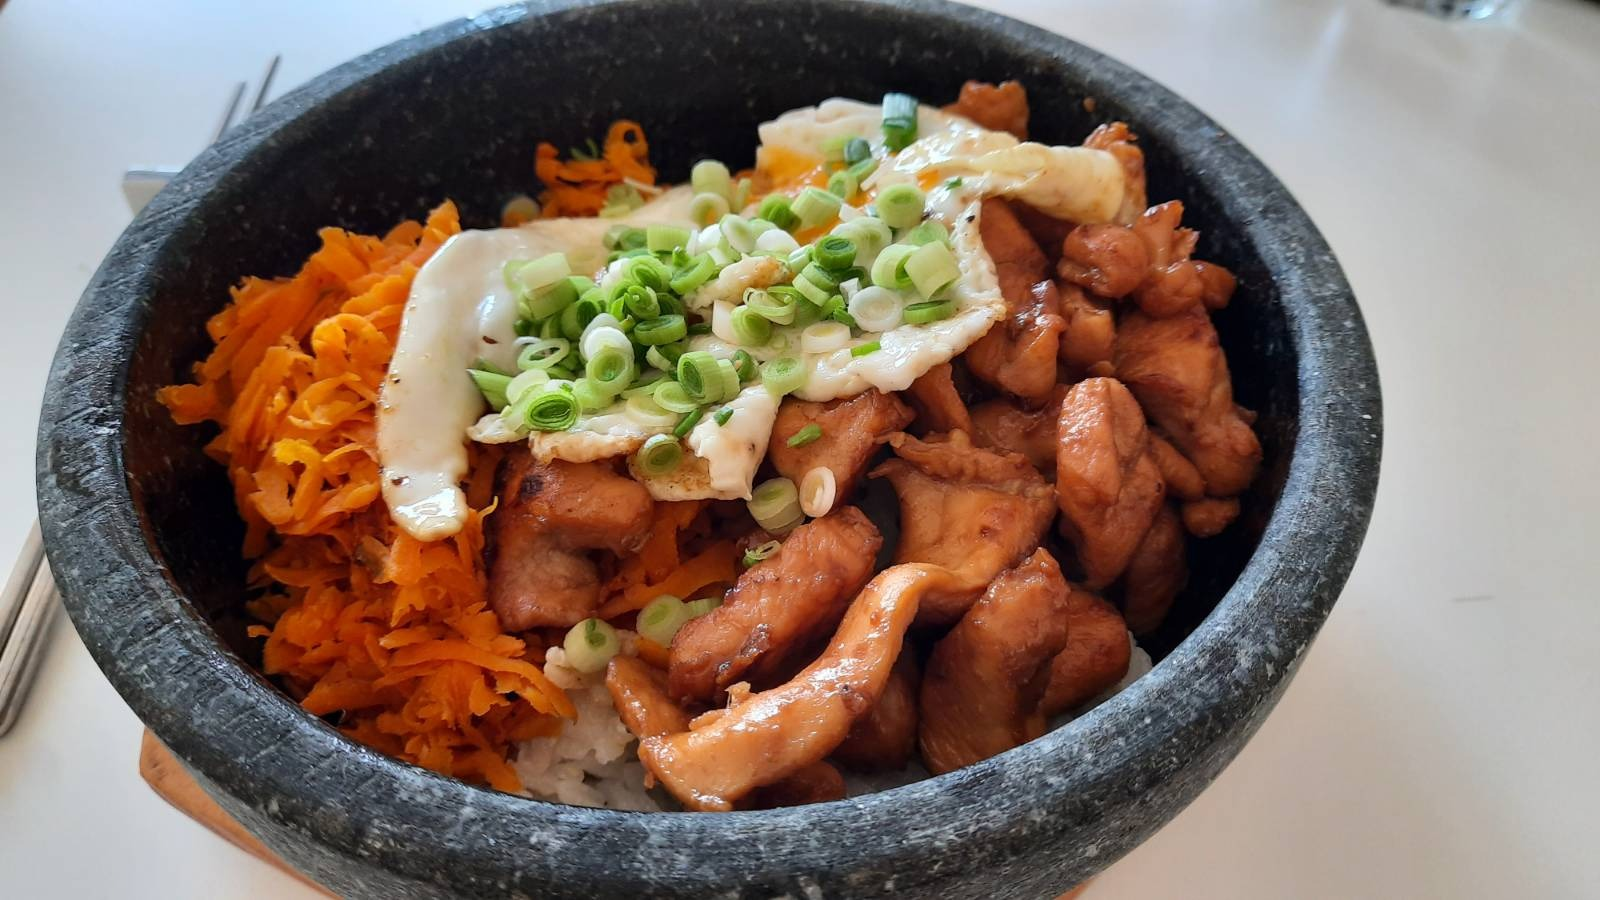
\includegraphics{images/teriyaki.jpeg}
\caption{FOTO}
\end{figure}

\hypertarget{ingredientes}{%
\section*{Ingredientes}\label{ingredientes}}
\addcontentsline{toc}{section}{Ingredientes}

\begin{itemize}
\tightlist
\item
  Muslo deshuesado o pechuga de pollo.
\item
  Huevo.
\item
  Zanahoria.
\item
  Ajo tierno.
\item
  Semillas de sésamo.
\item
  Arroz de grano corto.
\end{itemize}

Marinado del pollo:\footnote{ver también teriyaki rápido.}

\begin{itemize}
\tightlist
\item
  Salsa de soja.
\item
  Miel.
\item
  Sake.
\item
  Mirin.
\end{itemize}

\hypertarget{preparaciuxf3n}{%
\section*{Preparación}\label{preparaciuxf3n}}
\addcontentsline{toc}{section}{Preparación}

\begin{enumerate}
\def\labelenumi{\arabic{enumi}.}
\tightlist
\item
  Poner el \url{arroz} a cocer.
\item
  Cortar el pollo en pedazos pequeños. Preparar el marinado en un cuenco y dejar el pollo marinando mientras se prepara el resto.
\item
  Rallar la zanahoria y cortar el ajo tierno en rodajas muy finas.
\item
  En un wok a fuego alto, saltear la zanahoria con un poco de aceite, sal y bastante pimienta. Dejar apartado.
\item
  Con el mismo wok, saltear el pollo hasta que se quede sin líquido y empiece a tostarse el marinado.
\item
  En una sartén pequeña a fuego medio, freír un huevo con muy poco aceite.
\end{enumerate}

\hypertarget{pasta-carbonara}{%
\chapter{Pasta carbonara}\label{pasta-carbonara}}

\begin{figure}
\centering
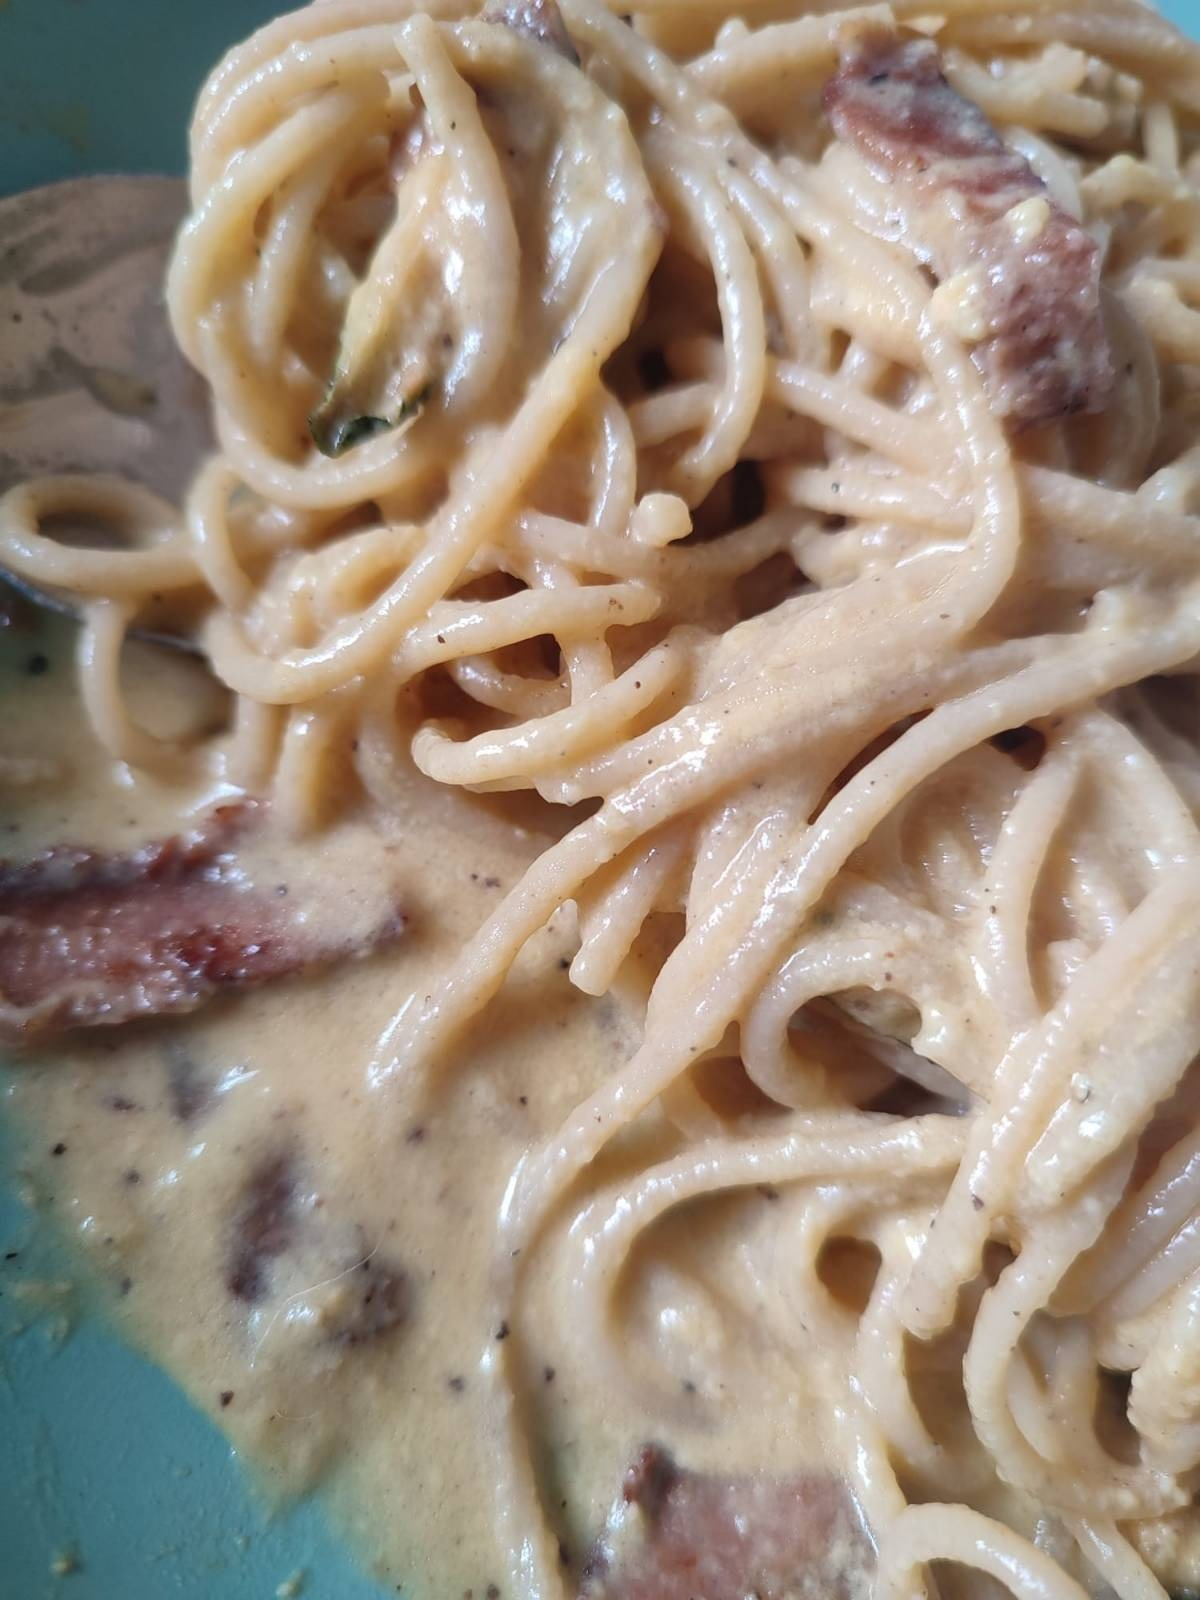
\includegraphics{images/carbonara.jpeg}
\caption{FOTO}
\end{figure}

\hypertarget{ingredientes-1}{%
\section*{Ingredientes}\label{ingredientes-1}}
\addcontentsline{toc}{section}{Ingredientes}

\begin{itemize}
\tightlist
\item
  Guanciale.\footnote{Se puede sustituir por panceta curada. El bacon es ahumado y cambia el sabor.}
\item
  Pasta (tortiglioni o spaghetti gruesos).
\item
  Pecorino o parmesano rallado.
\item
  1 huevo grande.
\end{itemize}

\hypertarget{preparaciuxf3n-1}{%
\section*{Preparación}\label{preparaciuxf3n-1}}
\addcontentsline{toc}{section}{Preparación}

\begin{enumerate}
\def\labelenumi{\arabic{enumi}.}
\tightlist
\item
  Poner la pasta a cocer siguiendo los tiempos del envase
\item
  Mientras se cuece la pasta, cortar el guanciale en tiras pequeñas y cocinarlas en una sartén a fuego bajo.
\item
  También a la vez, batir los huevos en un cuenco, y añadir suficiente queso hasta que la mezcla quede hecha una pasta densa. Añadir bastante pimienta.
\item
  Cuando la pasta esté casi lista, añadir unas cucharadas de agua de cocción de la pasta a la mezcla de huevo, queso y pimienta para hacerla menos densa.
\item
  Apagar el fuego del guanciale y echar la pasta en la sartén. No escurrir la pasta, echarla directamente desde la olla. Añadir más agua de cocción de pasta a la sartén hasta que haya una buena capa de líquido en el fondo.
\item
  Incorporar la mezcla de huevo, queso y pimienta en la pasta. Poner la sartén a fuego muy bajo y remover continuamente.
\item
  El agua de la pasta liga la mezcla y la hace más viscosa. Retirar del fuego y servir poco antes de que llegue a la viscosidad deseada.
\item
  Comer inmediatamente. En unos minutos será demasiado tarde para la salsa.
\end{enumerate}

\hypertarget{jeyuk-bokkeum}{%
\chapter{Jeyuk bokkeum}\label{jeyuk-bokkeum}}

!

\hypertarget{ingredientes-2}{%
\section*{Ingredientes}\label{ingredientes-2}}
\addcontentsline{toc}{section}{Ingredientes}

\begin{itemize}
\tightlist
\item
  Panceta de cerdo.\footnote{Se puede sustituir por muslo de pollo troceado, pero entonces el nombre del plato cambia.}
\item
  Zanahoria.
\item
  Cebolla.
\item
  Ajo tierno.
\item
  Caldo de verduras.
\item
  Semillas de sésamo.
\item
  Gochugaru.
\item
  Pimentón.
\item
  Harina de maíz.
\item
  Arroz de grano corto.
\end{itemize}

Marinado de la carne:

\begin{itemize}
\tightlist
\item
  Gochujang.
\item
  Ajo.
\item
  Salsa de soja.
\item
  Sake.
\item
  Mirin.
\item
  Aceite de sésamo.
\item
  Hoja de laurel.
\end{itemize}

\hypertarget{preparaciuxf3n-2}{%
\section*{Preparación}\label{preparaciuxf3n-2}}
\addcontentsline{toc}{section}{Preparación}

\begin{enumerate}
\def\labelenumi{\arabic{enumi}.}
\tightlist
\item
  Poner el \url{arroz} a cocer.
\item
  Cortar la panceta en lonchas finas. Es más fácil si se mete en el congelador durante un par de horas.
\item
  Marinar la carne un rato. La mezcla tiene que llevar bastante gochujang, mínimo una cucharada por persona.
\item
  Cortar la zanahoria y la cebolla en tiras finas, y picar el ajo tierno.
\item
  Saltear zanahoria y cebolla unos minutos.
\item
  Añadir carne y saltear a fuego fuerte. Añadir un poco de gochugaru y pimentón.
\item
  Cuando la carne esté medio hecha, añadir caldo.
\item
  Dejar que el caldo reduzca un poco, y espesar con harina de maíz. Servir cuando la salsa tenga la textura preferida.
\end{enumerate}

\hypertarget{hamburguesa-gringa}{%
\chapter{Hamburguesa Gringa}\label{hamburguesa-gringa}}

\begin{figure}
\centering
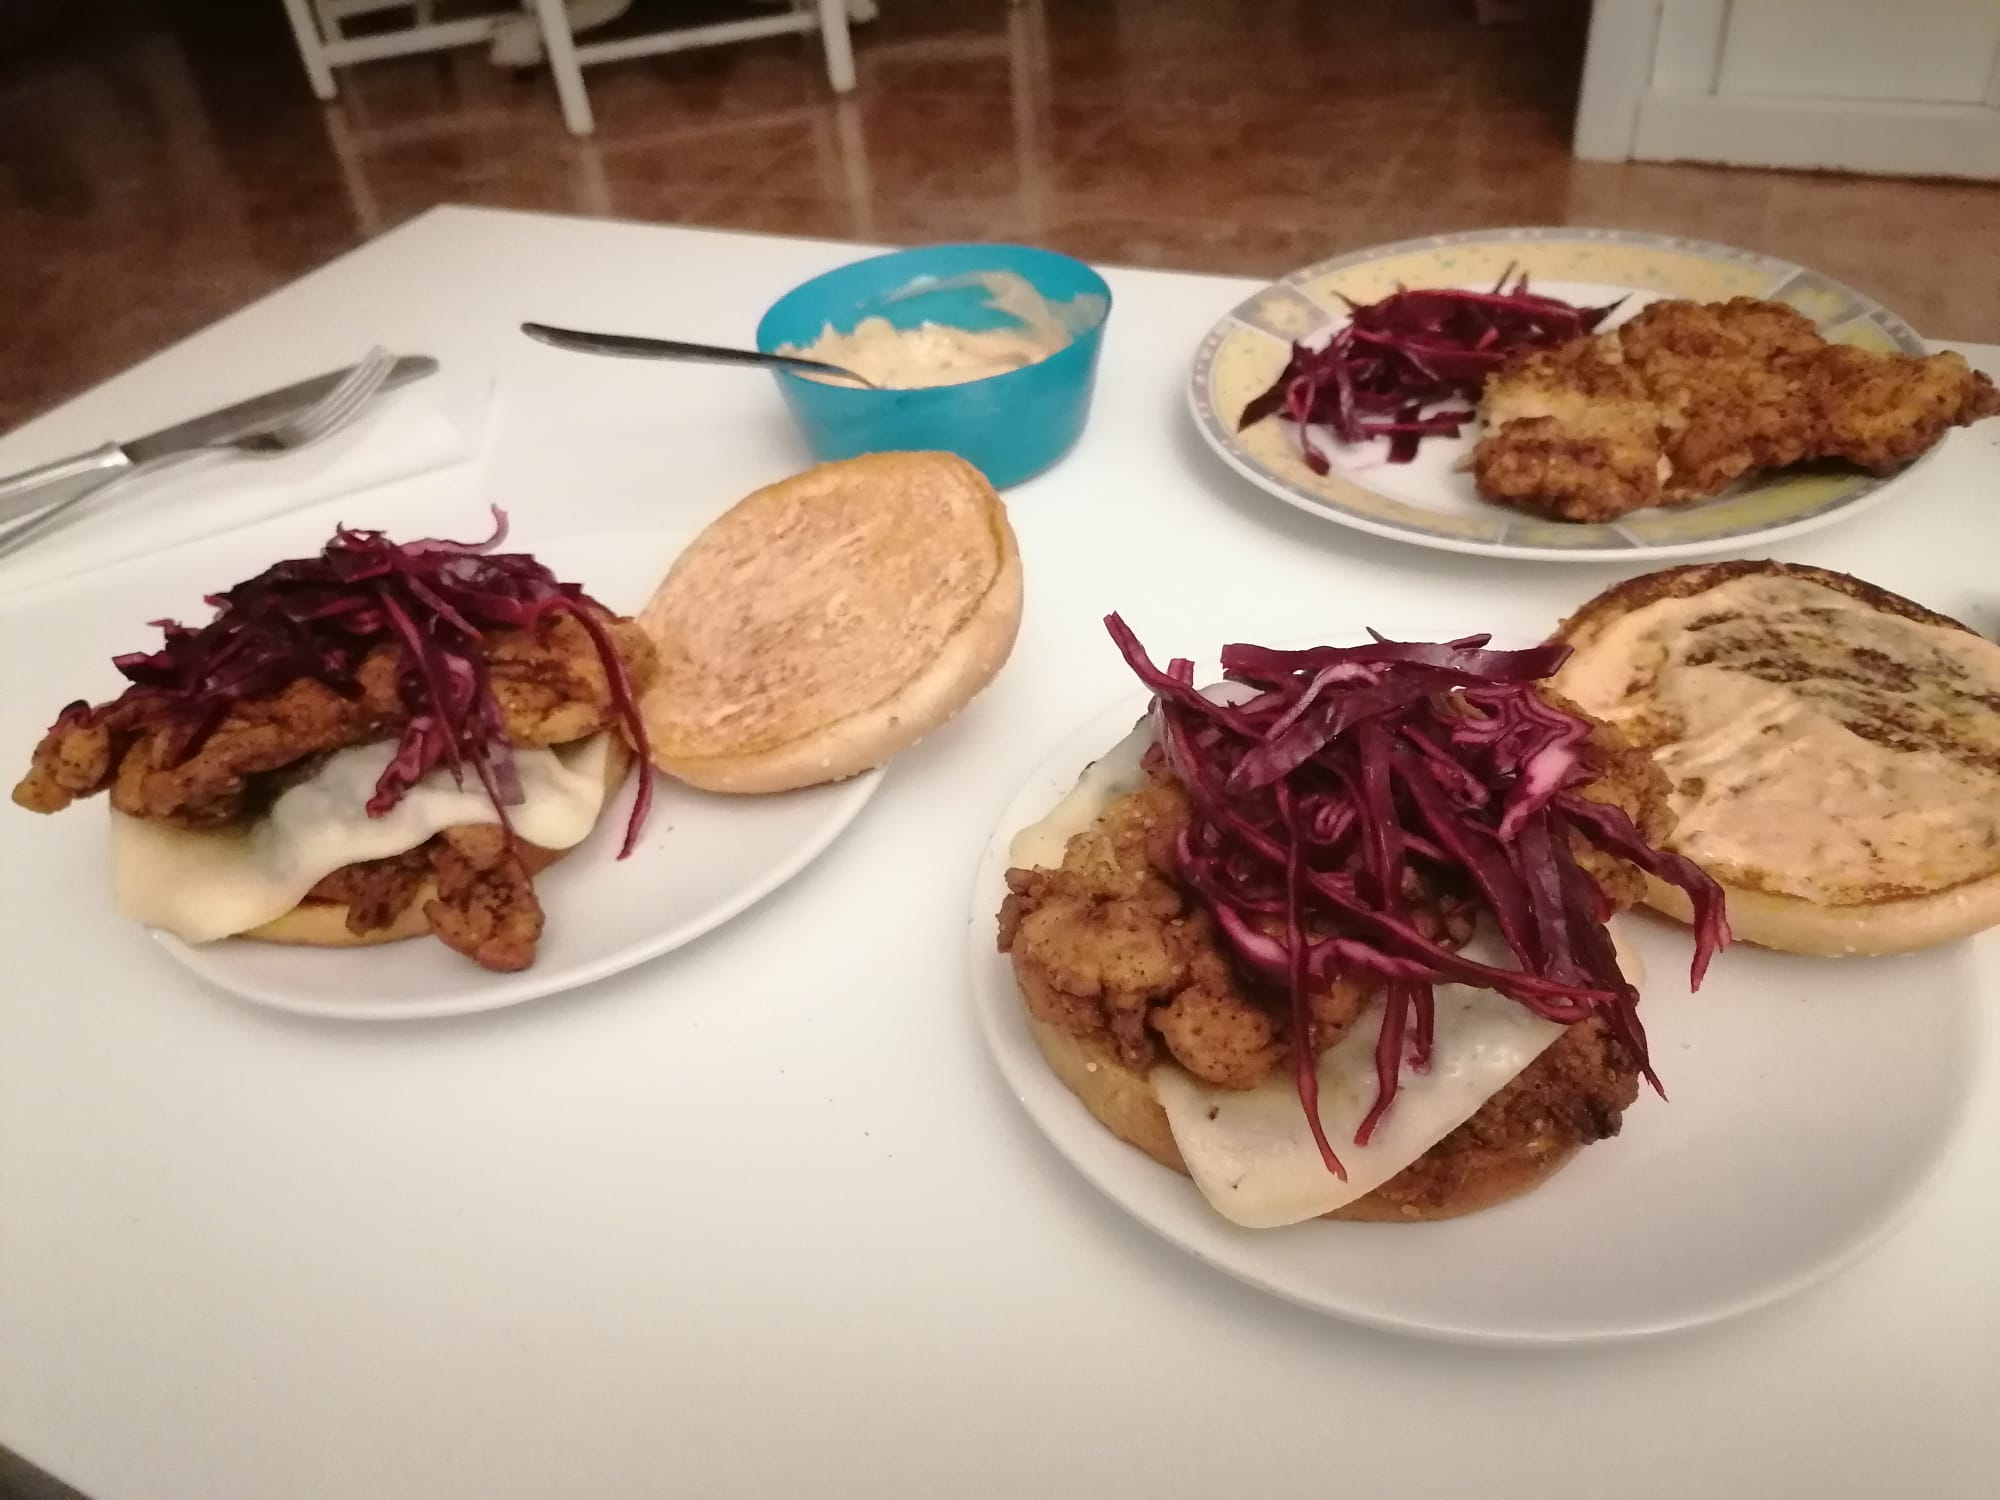
\includegraphics{images/gringa.jpg}
\caption{FOTO}
\end{figure}

\hypertarget{ingredientes-3}{%
\section*{Ingredientes}\label{ingredientes-3}}
\addcontentsline{toc}{section}{Ingredientes}

\begin{itemize}
\tightlist
\item
  Muslo de pollo.
\item
  Queso en lonchas.
\item
  Col lombarda.
\item
  Lima.
\item
  Pepinillos.
\item
  Cilantro.
\end{itemize}

Rebozado:

\begin{itemize}
\tightlist
\item
  Harina de trigo (70\%).
\item
  Harina de maíz (30\%).
\item
  Especias.\footnote{Usar una mezcla de todo lo que haya por casa (10 especias mínimo).}
\end{itemize}

Marinado:

\begin{itemize}
\tightlist
\item
  Leche
\item
  Zumo de limón
\item
  Huevo.
\item
  Especias.
\end{itemize}

Salsa:

\begin{itemize}
\tightlist
\item
  Mayonesa.
\item
  Miel.
\item
  \href{}{Chipotles en adobo}.
\end{itemize}

\hypertarget{preparaciuxf3n-3}{%
\section*{Preparación}\label{preparaciuxf3n-3}}
\addcontentsline{toc}{section}{Preparación}

\begin{enumerate}
\def\labelenumi{\arabic{enumi}.}
\tightlist
\item
  Marinar el pollo desde el día anterior.
\item
  Rebozar y freír el pollo en aceite de girasol muy caliente.
\item
  Mientras tanto, tostar el pan y preparar la salsa.
\item
  Cortar la col lombarda fina y echarle un poco de zumo de lima.
\item
  Untar el pan con la mayonesa de chipotle y montar la hamburguesa.
\end{enumerate}

\begin{quote}
\hypertarget{falafel}{%
\chapter{Falafel}\label{falafel}}
\end{quote}

\begin{quote}
\hypertarget{goulash}{%
\chapter{Goulash}\label{goulash}}
\end{quote}

\hypertarget{jeongol}{%
\chapter{Jeongol}\label{jeongol}}

\hypertarget{ingredientes-4}{%
\section*{Ingredientes}\label{ingredientes-4}}
\addcontentsline{toc}{section}{Ingredientes}

\begin{itemize}
\tightlist
\item
  Carne de ternera.
\item
  Fideos de boniato.
\item
  Enoki.
\item
  Zanahoria.
\item
  Ajo tierno.
\item
  Caldo.
\end{itemize}

Marinado de la carne:

\begin{itemize}
\tightlist
\item
  Salsa de soja.
\item
  Aceite de sésamo.
\item
  Sake.
\item
  Mirin.
\item
  Ajo picado.
\end{itemize}

\hypertarget{preparaciuxf3n-4}{%
\section*{Preparación}\label{preparaciuxf3n-4}}
\addcontentsline{toc}{section}{Preparación}

\begin{enumerate}
\def\labelenumi{\arabic{enumi}.}
\tightlist
\item
  Cortar la carne en tiras finas y dejar marinando, si es posible desde el día anterior.
\item
  Cortar las verduras en tiras finas. Cortar la base de los enoki y separarlos un poco.
\item
  En una olla a fuego fuerte, calentar el caldo y añadirle un poco de la misma mezcla que se usa para marinar la carne.
\item
  Meter en otra olla los fideos, carne y verduras crudas. Cuando el caldo esté listo, echar el caldo sobre la carne y verduras, y cocinar a fuego medio durante unos minutos, hasta que la carne esté cocinada y los fideos rehidratados.
\end{enumerate}

\hypertarget{bibimbap}{%
\chapter{Bibimbap}\label{bibimbap}}

\hypertarget{ingredientes-5}{%
\section*{Ingredientes}\label{ingredientes-5}}
\addcontentsline{toc}{section}{Ingredientes}

\begin{itemize}
\tightlist
\item
  Carne de ternera (opcional).
\item
  Huevo.
\item
  Zanahoria
\item
  Ajo tierno.
\item
  Pimiento verde.
\item
  Pimiento rojo.
\item
  Calabacín.
\item
  Cualquier verdura que haya por casa.
\item
  Arroz de grano corto.
\end{itemize}

Marinado de la carne:

\begin{itemize}
\tightlist
\item
  Salsa de soja.
\item
  Aceite de sésamo.
\item
  Sake.
\item
  Mirin.
\item
  Ajo picado.
\end{itemize}

Salsa:

\begin{itemize}
\tightlist
\item
  Gochujang.
\item
  Vinagre de arroz.
\end{itemize}

\hypertarget{preparaciuxf3n-5}{%
\section*{Preparación}\label{preparaciuxf3n-5}}
\addcontentsline{toc}{section}{Preparación}

\begin{enumerate}
\def\labelenumi{\arabic{enumi}.}
\tightlist
\item
  Cortar la carne en tiras finas y dejar marinando, si es posible desde el día anterior.
\item
  Poner a cocer arroz en blanco.
\item
  Cortar todas las verduras de la misma forma.
\item
  Saltear las verduras en un wok a fuego fuerte. Para más de dos raciones, saltear las verduras de una en una para que el wok no se llene demasiado.
\item
  Saltear la carne en el mismo wok y hacer un huevo a la plancha. Servir todo sobre el arroz.
\item
  Preparar la salsa. Si está muy espesa, añadir agua. Servir aparte para que la peña se eche la cantidad que quiera en su plato.
\end{enumerate}

\hypertarget{japchae}{%
\chapter{Japchae}\label{japchae}}

\begin{figure}
\centering
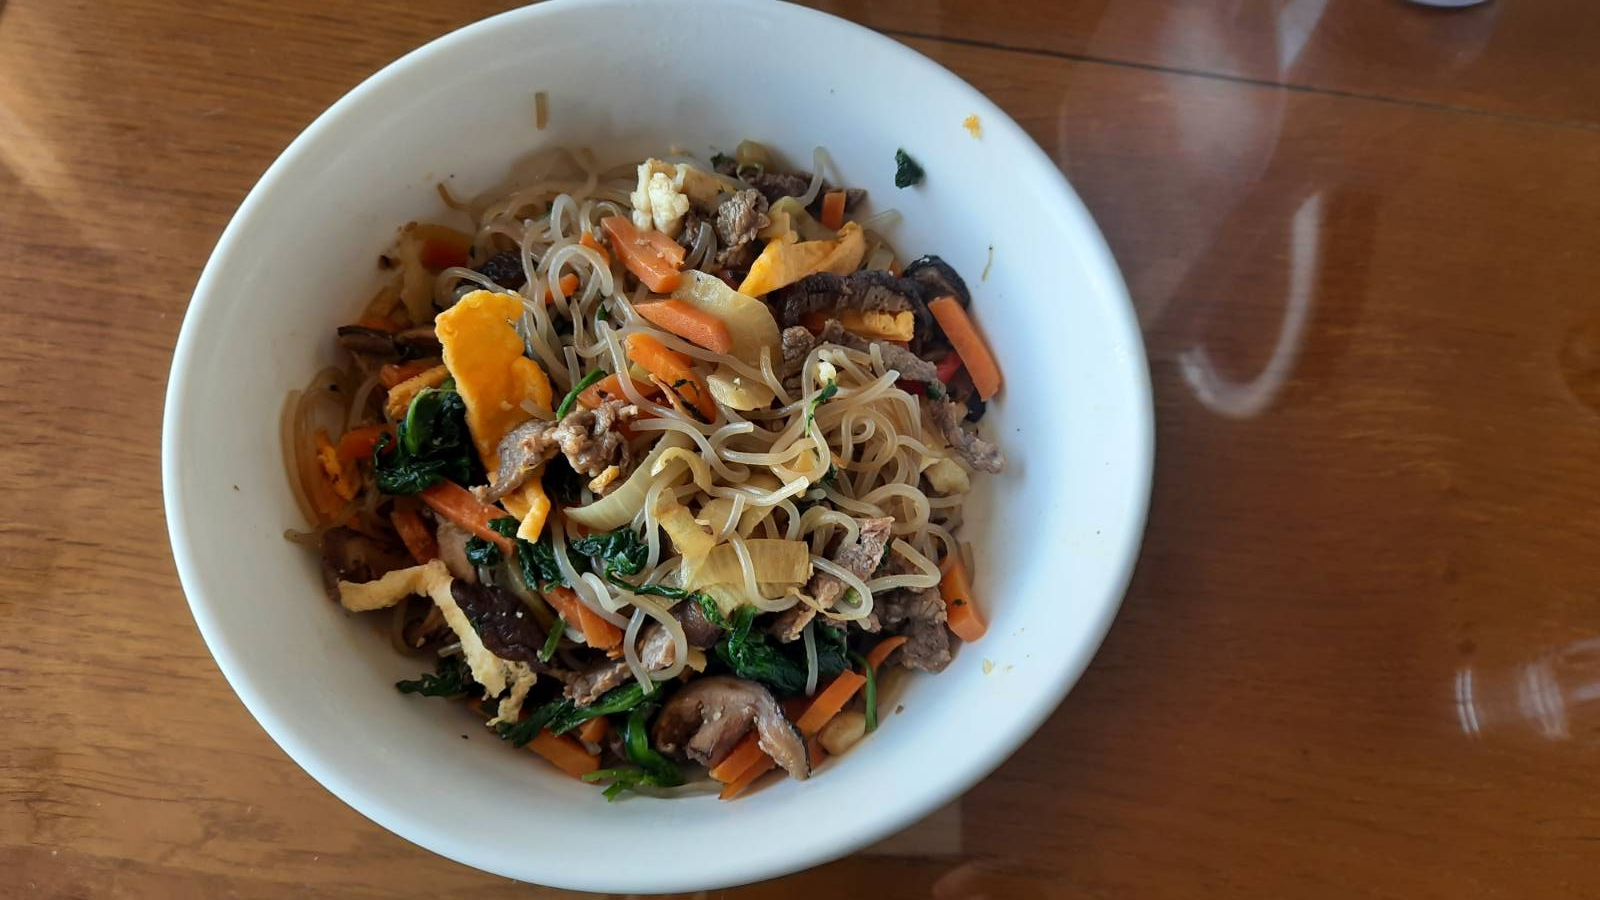
\includegraphics{images/japchae.jpg}
\caption{FOTO}
\end{figure}

\hypertarget{ingredientes-6}{%
\section*{Ingredientes}\label{ingredientes-6}}
\addcontentsline{toc}{section}{Ingredientes}

\begin{itemize}
\tightlist
\item
  Carne de ternera (opcional).
\item
  Huevo.
\item
  Zanahoria.
\item
  Cebolla.
\item
  Pimiento.
\item
  Espinacas.
\item
  Aceite de sésamo.
\item
  Panela.
\end{itemize}

Marinado de la carne:

\begin{itemize}
\tightlist
\item
  Salsa de soja.
\item
  Aceite de sésamo.
\item
  Sake.
\item
  Mirin.
\item
  Ajo picado.
\end{itemize}

\hypertarget{preparaciuxf3n-6}{%
\section*{Preparación}\label{preparaciuxf3n-6}}
\addcontentsline{toc}{section}{Preparación}

\begin{enumerate}
\def\labelenumi{\arabic{enumi}.}
\tightlist
\item
  Cortar la carne en tiras finas y dejar marinando, si es posible desde el día anterior.
\item
  Hervir las espinacas, estrujar para quitarles el agua y añadir un poco de aceite de sésamo.
\item
  Separar la clara y yema del huevo. Batir por separado y hacer una tortilla con cada una. Cortar ambas en tiras finas.
\item
  Cortar el resto de las verduras en tiras finas.
\item
  Saltear las verduras en un wok a fuego fuerte.
\item
  Saltear la carne en el mismo wok.
\item
  Hervir los fideos de boniato hasta que estén comestibles, y escurrir.
\item
  En un bol grande, combinar salsa de soja, aceite de sésamo y panela. Añadir todos los ingredientes cocinados, y mezclar bien.
\end{enumerate}

\hypertarget{ajitama}{%
\chapter{Ajitama}\label{ajitama}}

!

\hypertarget{ingredientes-7}{%
\section*{Ingredientes}\label{ingredientes-7}}
\addcontentsline{toc}{section}{Ingredientes}

\begin{itemize}
\tightlist
\item
  Huevos.
\item
  Salsa de soja.
\item
  Azúcar.
\end{itemize}

\hypertarget{preparaciuxf3n-7}{%
\section*{Preparación}\label{preparaciuxf3n-7}}
\addcontentsline{toc}{section}{Preparación}

\begin{enumerate}
\def\labelenumi{\arabic{enumi}.}
\tightlist
\item
  En una olla, calentar agua hasta que hierva.
\item
  Sumergir los huevos en agua hirviendo durante 6 minutos y medio.
\item
  Sacar los huevos del agua y cortar la cocción con agua fría o hielo.
\item
  Para el marinado, mezclar la misma cantidad de agua y salsa de soja, y unas cucharadas de azúcar.
\item
  Pelar los huevos y dejarlos marinando toda la noche.
\end{enumerate}

\hypertarget{caldo-ruxe1pido-para-ramen}{%
\chapter{Caldo rápido para ramen}\label{caldo-ruxe1pido-para-ramen}}

!

\hypertarget{ingredientes-8}{%
\section*{Ingredientes}\label{ingredientes-8}}
\addcontentsline{toc}{section}{Ingredientes}

\begin{itemize}
\tightlist
\item
  Caldo de puchero Aneto.
\item
  Salsa de soja.
\item
  Sake.
\item
  Mirin.
\item
  Ajos.
\item
  Aceite de sésamo.
\item
  (opcional) Escamas de bonito.
\item
  (opcional) Guindillas.
\end{itemize}

\hypertarget{preparaciuxf3n-8}{%
\section*{Preparación}\label{preparaciuxf3n-8}}
\addcontentsline{toc}{section}{Preparación}

\begin{enumerate}
\def\labelenumi{\arabic{enumi}.}
\tightlist
\item
  En una olla, mezclar un poco de salsa de soja, ajo, sake y mirin, y dejar que se cocinen a fuego medio durante unos minutos.
\item
  Añadir el caldo, subir el fuego y cocinar durante un rato.
\item
  Añadir el aceite de sésamo y cocinar unos minutos más.
\end{enumerate}

\begin{quote}
\hypertarget{wok-noodles}{%
\chapter{Wok noodles}\label{wok-noodles}}
\end{quote}

\hypertarget{naan}{%
\chapter{Naan}\label{naan}}

!

\hypertarget{ingredientes-9}{%
\section*{Ingredientes}\label{ingredientes-9}}
\addcontentsline{toc}{section}{Ingredientes}

\begin{itemize}
\tightlist
\item
  Harina.
\item
  Yogur.
\item
  Levadura.
\item
  Sal.
\item
  Ajo.
\item
  Mantequilla.
\end{itemize}

\hypertarget{preparaciuxf3n-9}{%
\section*{Preparación}\label{preparaciuxf3n-9}}
\addcontentsline{toc}{section}{Preparación}

\begin{enumerate}
\def\labelenumi{\arabic{enumi}.}
\tightlist
\item
  Picar ajo. Calentar mantequilla en una sartén hasta que chisporrotee. En ese momento, apagar el fuego, añadir el ajo y remover.
\item
  En un bol grande, combinar agua templada, levadura y sal. Añadir un poco de mantequilla de la mezcla anterior.
\item
  Añadir harina (4 veces la cantidad de agua). Amasar hasta conseguir una masa homogénea, y amasar un poco más. Añadiri más harina o agua si hace falta.
\item
  Dejar reposar la masa un par de horas a temperatura ambiente. Cortar en trozos, tapar con un paño y dejar reposar quince minutos más. Extender las masas con un rodillo, hasta que estén bastante finas.
\item
  Calentar una sartén a fuego muy alto. Cuando esté muy caliente, esperar cinco minutos más. Tostar los naans un par de minutos por cada lado.
\item
  Al sacarlos de la sartén, añadir un poco de la mezcla de mantequilla y ajo a cada lado (recalentar la mezcla si ya se ha solidificado).
\end{enumerate}

\begin{quote}
\hypertarget{tikka-masala}{%
\chapter{Tikka masala}\label{tikka-masala}}
\end{quote}

\begin{quote}
\hypertarget{hummus}{%
\chapter{Hummus}\label{hummus}}
\end{quote}

\hypertarget{focaccia}{%
\chapter{Focaccia}\label{focaccia}}

\begin{figure}
\centering
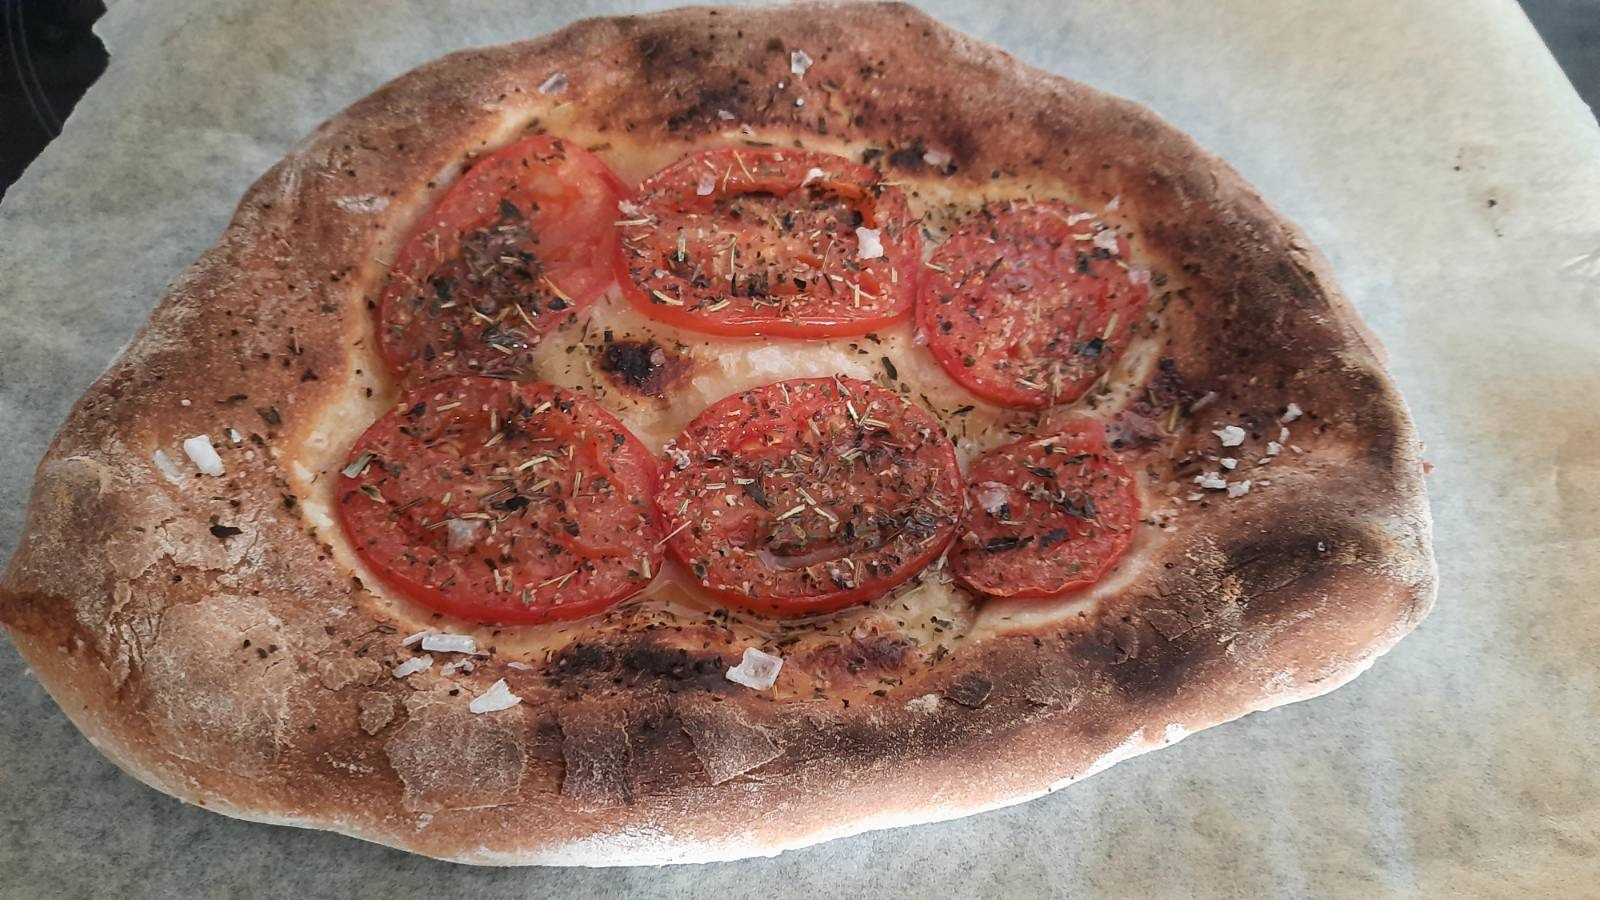
\includegraphics{images/focaccia.jpg}
\caption{FOTO}
\end{figure}

\hypertarget{ingredientes-10}{%
\section*{Ingredientes}\label{ingredientes-10}}
\addcontentsline{toc}{section}{Ingredientes}

\begin{itemize}
\tightlist
\item
  Harina.
\item
  Levadura.
\item
  Sal.
\item
  Azúcar.
\item
  Aceite de oliva.
\item
  Tomates.
\item
  Orégano.
\end{itemize}

\hypertarget{preparaciuxf3n-10}{%
\section*{Preparación}\label{preparaciuxf3n-10}}
\addcontentsline{toc}{section}{Preparación}

\begin{enumerate}
\def\labelenumi{\arabic{enumi}.}
\tightlist
\item
  En un bol, mezclar harina, levadura, sal y azúcar. Añadir, poco a poco y mientras se remueve, un 65\% de agua respecto a la cantidad de harina. Añadir un poco de aceite de oliva.
\item
  Amasar con las manos hasta que la masa esté totalmente homogénea, y luego un rato más. Es normal que esté un poco pegajosa porque tiene mucha agua.
\item
  Esperar hasta el día siguiente. Para hacer la receta hoy, tendrías que haber preparado la masa ayer.\footnote{Hay que espabilar.}
\item
  Al día siguiente, cortar la masa en raciones individuales. Extender la masa sin tocar el borde, extendiendo siempre la parte central.
\item
  Precalentar el horno en modo grill.
\item
  Encima de la masa, añadir unas rodajas de tomate, orégano, aceite de oliva, sal en escamas y pimienta.
\item
  Cocinar en el horno unos minutos, lo más cerca del grill que sea posible.
\end{enumerate}

\begin{quote}
\hypertarget{arroz-mexicano}{%
\chapter{Arroz mexicano}\label{arroz-mexicano}}
\end{quote}

\begin{quote}
\hypertarget{guacamole}{%
\chapter{Guacamole}\label{guacamole}}
\end{quote}

\begin{quote}
\hypertarget{nachos}{%
\chapter{Nachos}\label{nachos}}
\end{quote}

\hypertarget{filloas}{%
\chapter{Filloas}\label{filloas}}

\begin{figure}
\centering
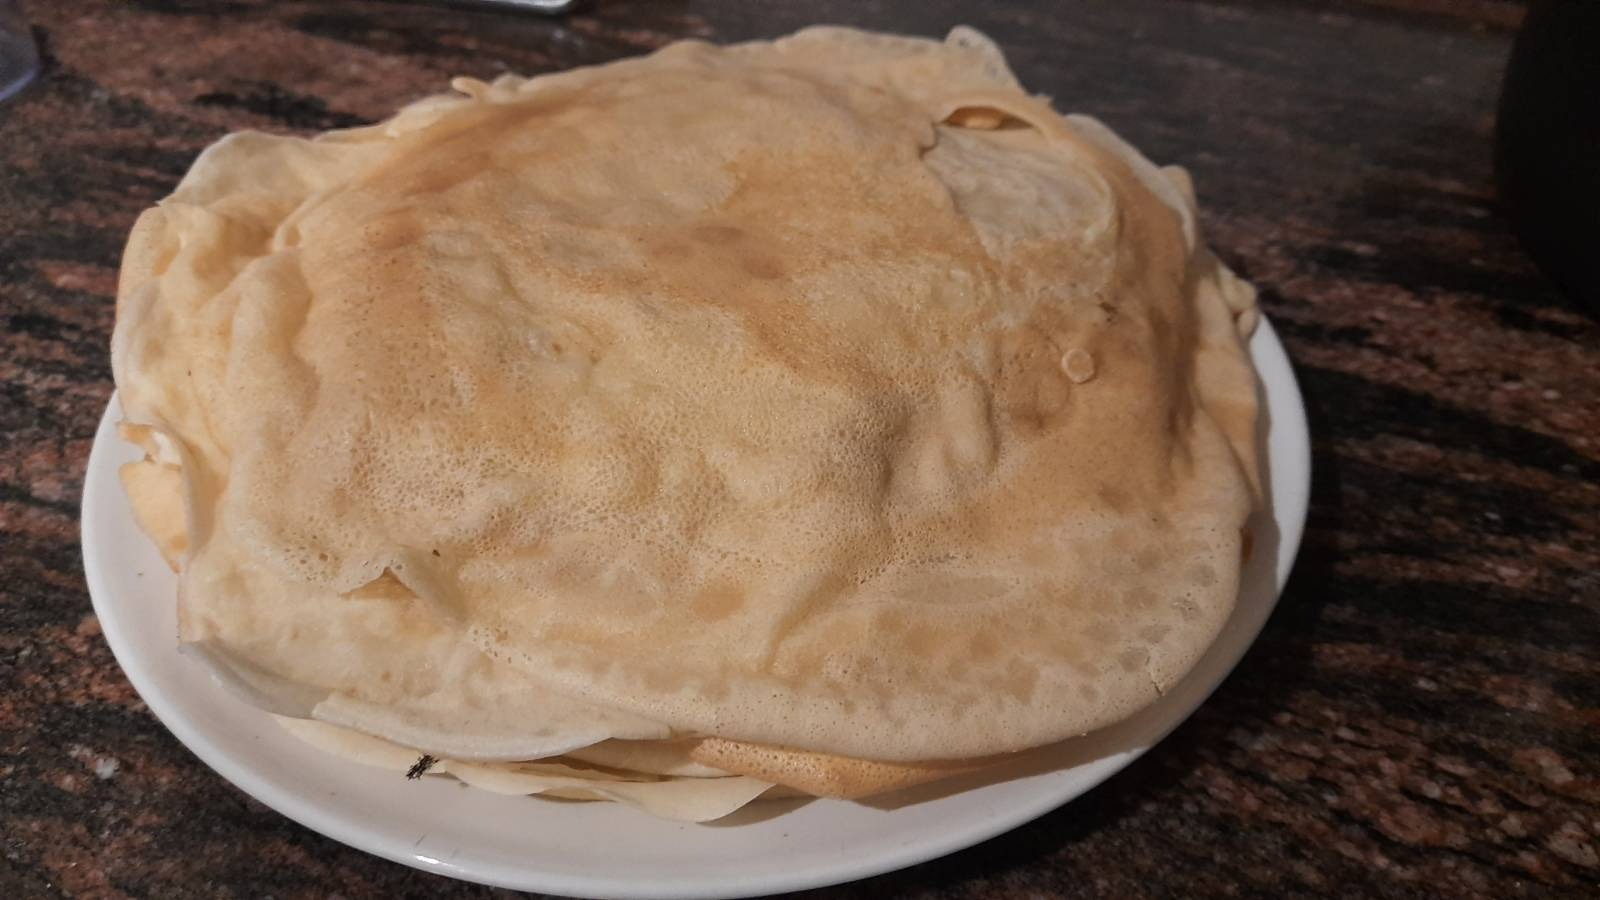
\includegraphics{images/filloas.jpeg}
\caption{FOTO}
\end{figure}

\begin{figure}
\centering
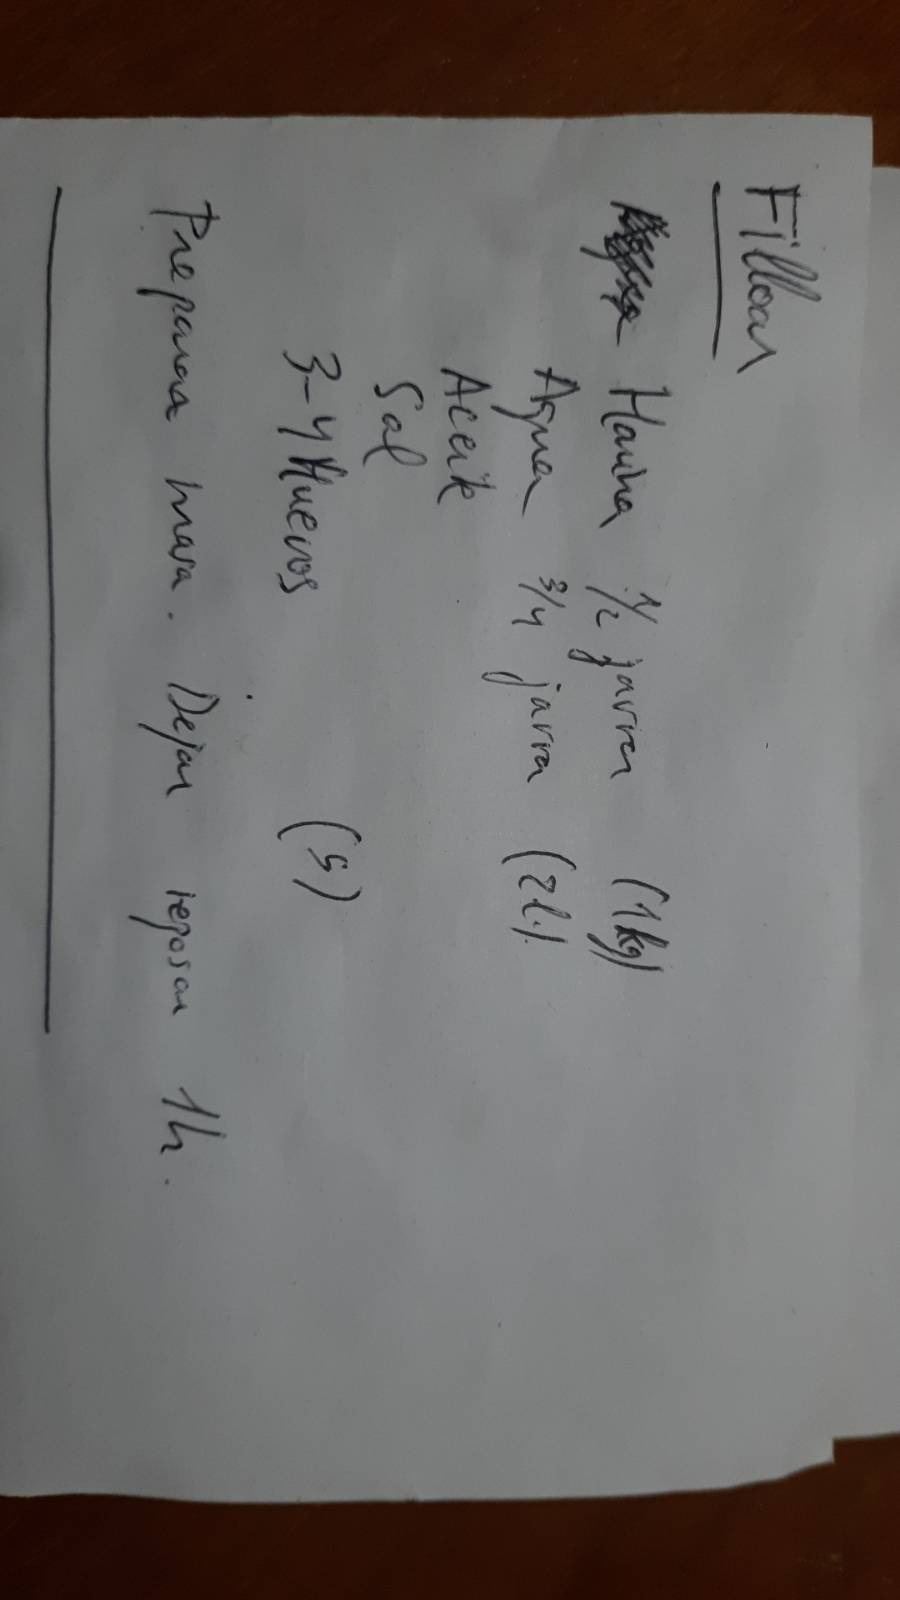
\includegraphics{images/filloas-receta.jpeg}
\caption{FOTO}
\end{figure}

\begin{quote}
\hypertarget{tarta-de-zanahoria}{%
\chapter{Tarta de zanahoria}\label{tarta-de-zanahoria}}
\end{quote}

\hypertarget{croquetas}{%
\chapter{Croquetas}\label{croquetas}}

\begin{figure}
\centering

\includegraphics{images/grogu.png}
\caption{FOTO}
\end{figure}

\hypertarget{encurtidos}{%
\chapter{Encurtidos}\label{encurtidos}}

\begin{figure}
\centering
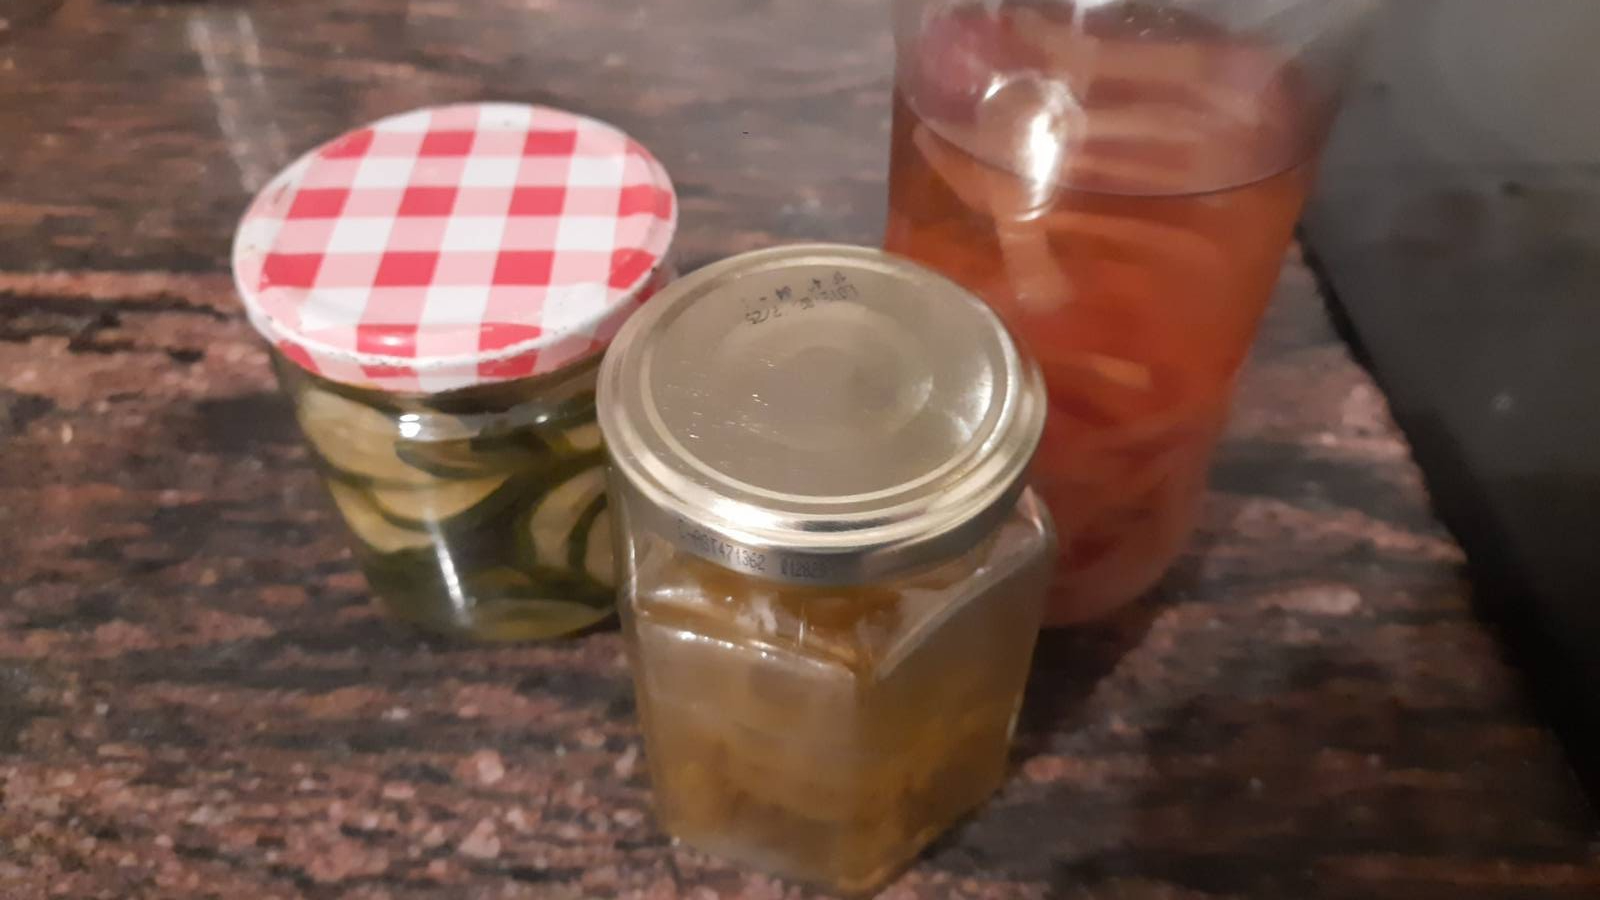
\includegraphics{images/encurtidos.jpg}
\caption{FOTO}
\end{figure}

\hypertarget{ingredientes-11}{%
\section*{Ingredientes}\label{ingredientes-11}}
\addcontentsline{toc}{section}{Ingredientes}

\begin{itemize}
\tightlist
\item
  Cualquier cosa.
\item
  Vinagre de vino blanco.
\item
  Panela.
\end{itemize}

\hypertarget{preparaciuxf3n-11}{%
\section*{Preparación}\label{preparaciuxf3n-11}}
\addcontentsline{toc}{section}{Preparación}

\begin{enumerate}
\def\labelenumi{\arabic{enumi}.}
\tightlist
\item
  En una olla, echar un vaso y medio de agua por cada vaso de vinagre. Añadir una o dos cucharadas de azúcar.
\item
  Hervir la mezcla unos minutos, y echar sobre cualquier cosa.
\item
  No es una conserva de verdad. Aguanta unas semanas, o meses como mucho, en la nevera.
\end{enumerate}

\hypertarget{salsa-de-tomate-asado}{%
\chapter{Salsa de tomate asado}\label{salsa-de-tomate-asado}}

\begin{figure}
\centering
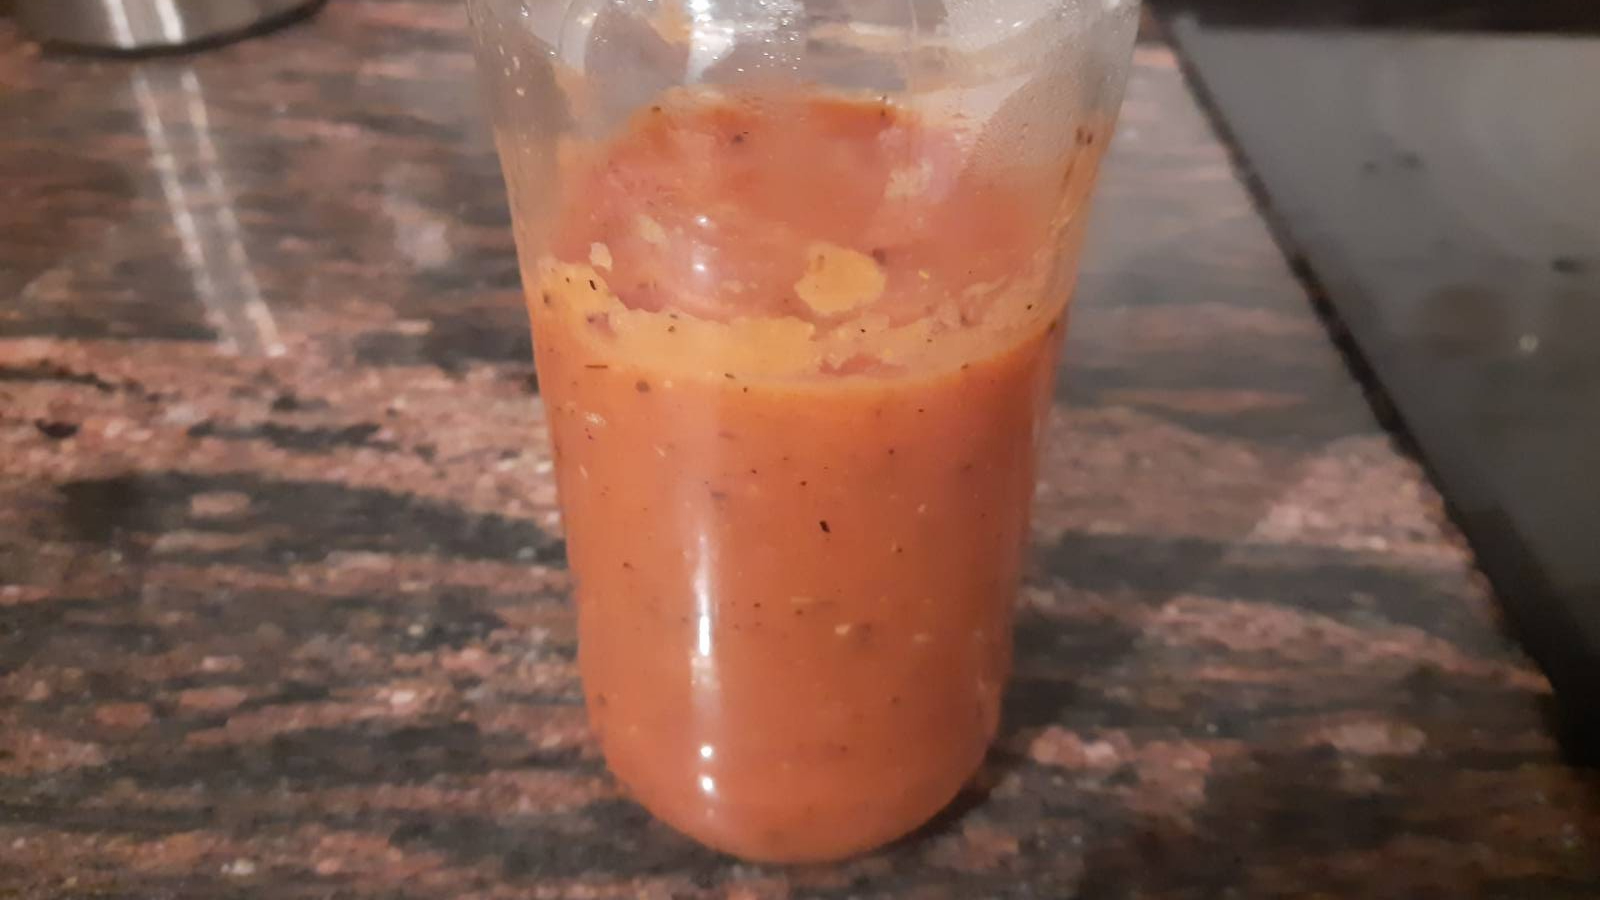
\includegraphics{images/salsa-de-tomate-asado.jpg}
\caption{FOTO}
\end{figure}

\hypertarget{ingredientes-12}{%
\section*{Ingredientes}\label{ingredientes-12}}
\addcontentsline{toc}{section}{Ingredientes}

\begin{itemize}
\tightlist
\item
  Tomates.
\item
  Cebolla.
\item
  Ajos.
\end{itemize}

\hypertarget{preparaciuxf3n-12}{%
\section*{Preparación}\label{preparaciuxf3n-12}}
\addcontentsline{toc}{section}{Preparación}

\begin{enumerate}
\def\labelenumi{\arabic{enumi}.}
\tightlist
\item
  Precalentar el grill del horno.
\item
  Cortar unos pocos tomates y media cebolla en dos o tres trozos por cada pieza. Aplastar unos ajos (sin quitarles la piel).
\item
  Poner todo, con un poco de sal y aceite, en una bandeja de horno, y dejar bajo el grill unos 10 minutos. Es importante que la bandeja esté lo más pegada al grill que sea posible.
\item
  Esperar a que los tomates estén un poco negros. Cuando creas que ya están, les faltan cinco minutos.
\item
  Triturar todo con una batidora.
\end{enumerate}

  \bibliography{book.bib,packages.bib}

\end{document}
